% This is "sig-alternate.tex" V2.1 April 2013
% This file should be compiled with V2.5 of "sig-alternate.cls" May 2012
%
% This example file demonstrates the use of the 'sig-alternate.cls'
% V2.5 LaTeX2e document class file. It is for those submitting
% articles to ACM Conference Proceedings WHO DO NOT WISH TO
% STRICTLY ADHERE TO THE SIGS (PUBS-BOARD-ENDORSED) STYLE.
% The 'sig-alternate.cls' file will produce a similar-looking,
% albeit, 'tighter' paper resulting in, invariably, fewer pages.
%
% ----------------------------------------------------------------------------------------------------------------
% This .tex file (and associated .cls V2.5) produces:
%       1) The Permission Statement
%       2) The Conference (location) Info information
%       3) The Copyright Line with ACM data
%       4) NO page numbers
%
% as against the acm_proc_article-sp.cls file which
% DOES NOT produce 1) thru' 3) above.
%
% Using 'sig-alternate.cls' you have control, however, from within
% the source .tex file, over both the CopyrightYear
% (defaulted to 200X) and the ACM Copyright Data
% (defaulted to X-XXXXX-XX-X/XX/XX).
% e.g.
% \CopyrightYear{2007} will cause 2007 to appear in the copyright line.
% \crdata{0-12345-67-8/90/12} will cause 0-12345-67-8/90/12 to appear in the copyright line.
%
% ---------------------------------------------------------------------------------------------------------------
% This .tex source is an example which *does* use
% the .bib file (from which the .bbl file % is produced).
% REMEMBER HOWEVER: After having produced the .bbl file,
% and prior to final submission, you *NEED* to 'insert'
% your .bbl file into your source .tex file so as to provide
% ONE 'self-contained' source file.
%
% ================= IF YOU HAVE QUESTIONS =======================
% Questions regarding the SIGS styles, SIGS policies and
% procedures, Conferences etc. should be sent to
% Adrienne Griscti (griscti@acm.org)
%
% Technical questions _only_ to
% Gerald Murray (murray@hq.acm.org)
% ===============================================================
%
% For tracking purposes - this is V2.0 - May 2012

\documentclass{sig-alternate-05-2015}
\usepackage{color}

\begin{document}

% Copyright
\setcopyright{acmcopyright}
%\setcopyright{acmlicensed}
%\setcopyright{rightsretained}
%\setcopyright{usgov}
%\setcopyright{usgovmixed}
%\setcopyright{cagov}
%\setcopyright{cagovmixed}


% DOI
\doi{10.475/123_4} 

% ISBN
\isbn{123-4567-24-567/08/06}

%Conference
\conferenceinfo{PLDI '13}{June 16--19, 2013, Seattle, WA, USA}

\acmPrice{\$15.00}

%
% --- Author Metadata here ---
\conferenceinfo{WOODSTOCK}{'97 El Paso, Texas USA}
%\CopyrightYear{2007} % Allows default copyright year (20XX) to be over-ridden - IF NEED BE.
%\crdata{0-12345-67-8/90/01}  % Allows default copyright data (0-89791-88-6/97/05) to be over-ridden - IF NEED BE.
% --- End of Author Metadata ---

\title{YouUnderstood.me? Readability-based retrieval of reading materials for students and educators}

%
% You need the command \numberofauthors to handle the 'placement
% and alignment' of the authors beneath the title.
%
% For aesthetic reasons, we recommend 'three authors at a time'
% i.e. three 'name/affiliation blocks' be placed beneath the title.
%
% NOTE: You are NOT restricted in how many 'rows' of
% "name/affiliations" may appear. We just ask that you restrict
% the number of 'columns' to three.
%
% Because of the available 'opening page real-estate'
% we ask you to refrain from putting more than six authors
% (two rows with three columns) beneath the article title.
% More than six makes the first-page appear very cluttered indeed.
%
% Use the \alignauthor commands to handle the names
% and affiliations for an 'aesthetic maximum' of six authors.
% Add names, affiliations, addresses for
% the seventh etc. author(s) as the argument for the
% \additionalauthors command.
% These 'additional authors' will be output/set for you
% without further effort on your part as the last section in
% the body of your article BEFORE References or any Appendices.

\numberofauthors{2} %  in this sample file, there are a *total*
% of EIGHT authors. SIX appear on the 'first-page' (for formatting
% reasons) and the remaining two appear in the \additionalauthors section.
%
\author{
% You can go ahead and credit any number of authors here,
% e.g. one 'row of three' or two rows (consisting of one row of three
% and a second row of one, two or three).
%
% The command \alignauthor (no curly braces needed) should
% precede each author name, affiliation/snail-mail address and
% e-mail address. Additionally, tag each line of
% affiliation/address with \affaddr, and tag the
% e-mail address with \email.
%
% 1st. author
\alignauthor
Ion Madrazo\\
       \affaddr{Computer Science Department}\\
       \affaddr{Boise State University}\\
       \affaddr{Boise, Idaho, USA}\\
       \email{ionmadrazo@boisestate.edu}
% 2nd. author
\alignauthor
Sole Pera\\
       \affaddr{Computer Science Department}\\
       \affaddr{Boise State University}\\
       \affaddr{Boise, Idaho, USA}\\
       \email{solepera@boisestate.edu}
}
% There's nothing stopping you putting the seventh, eighth, etc.
% author on the opening page (as the 'third row') but we ask,
% for aesthetic reasons that you place these 'additional authors'
% in the \additional authors block, viz.

\date{30 July 1999}
% Just remember to make sure that the TOTAL number of authors
% is the number that will appear on the first page PLUS the
% number that will appear in the \additionalauthors section.

\maketitle
\begin{abstract}


K-12 students and educators make use of online resources to fulfill their academic information needs on a daily basis. Unfortunately, they are forced to spend a large amount of time seeking for adequate materials. In the case of the students, they can often get discouraged because the contents they retrieve are outside their comprehension level, whether being too easy or too difficult  for them to read. For educators, finding materials for curriculum development that suit the students' reading abilities can also be challenging.  In this paper, we present \textit{YouUnderstood.me}, a web application that makes use of natural language processing, machine learning and information retrieval techniques to help both students and educators in the process of finding materials that fit the reading skills of each individual student in a faster and more efficient way. \textit{YouUnderstood.me} combines: (1) a search interface that by joining a search engine and a readability formula, permits the fast retrieval of documents from different sources, (2)  a readability tracking system that enables the aforementioned stakeholders to see which the reading skills of individual students are  and (3) an analysis tool that enables educators to analyze specific reading materials found outside \textit{YouUnderstood.me}.






\end{abstract}


%
% The code below should be generated by the tool at
% http://dl.acm.org/ccs.cfm
% Please copy and paste the code instead of the example below. 
%



 \begin{CCSXML}
<ccs2012>
<concept>
<concept_id>10002951.10003317.10003331.10003271</concept_id>
<concept_desc>Information systems~Personalization</concept_desc>
<concept_significance>500</concept_significance>
</concept>
<concept>
<concept_id>10002951.10003317.10003331.10003336</concept_id>
<concept_desc>Information systems~Search interfaces</concept_desc>
<concept_significance>500</concept_significance>
</concept>
<concept>
<concept_id>10002951.10003317.10003347.10003356</concept_id>
<concept_desc>Information systems~Clustering and classification</concept_desc>
<concept_significance>300</concept_significance>
</concept>
<concept>
<concept_id>10010147.10010178.10010179</concept_id>
<concept_desc>Computing methodologies~Natural language processing</concept_desc>
<concept_significance>500</concept_significance>
</concept>
</ccs2012>
\end{CCSXML}

\ccsdesc[500]{Information systems~Personalization}
\ccsdesc[500]{Information systems~Search interfaces}
\ccsdesc[300]{Information systems~Clustering and classification}
\ccsdesc[500]{Computing methodologies~Natural language processing}





%
% End generated code
%

%
%  Use this command to print the description
%
\printccsdesc

% We no longer use \terms command
%\terms{Theory}

\keywords{Search engines; Filtering; Readability assessment; Student tracking}


\begin{figure*}[ht]
 \centering
  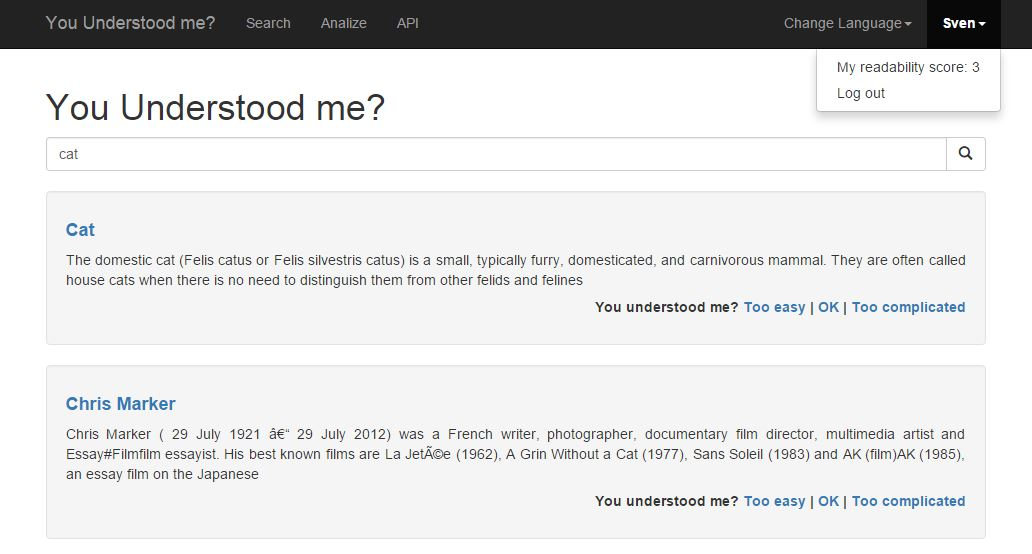
\includegraphics[width=1\textwidth]{SearchEngineStudent}
 \caption{Screenshot of the search interface for students}
 \label{fig:studentSearch}
 \end{figure*}



\begin{figure*}[ht]
 \centering
  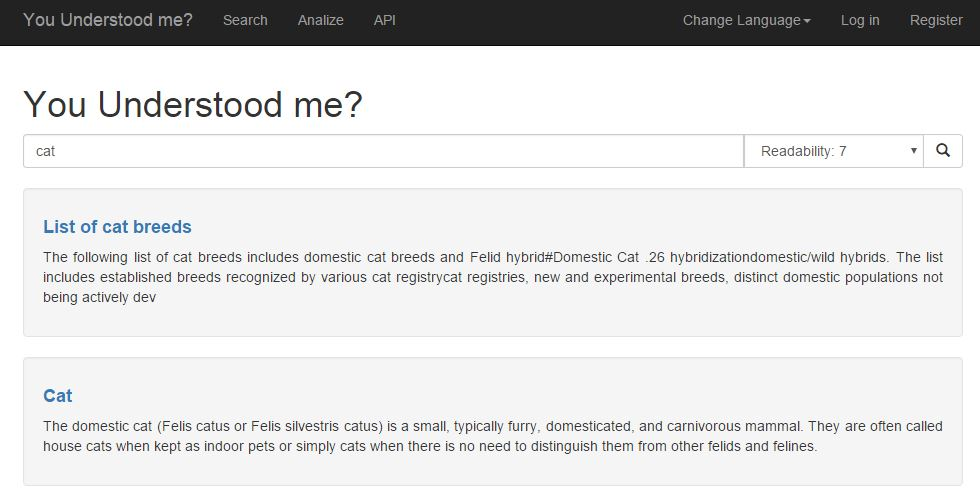
\includegraphics[width=1\textwidth]{SearchEngineEducator}
 \caption{Screenshot of the search interface for educators}
  \label{fig:educatorSearch}
 \end{figure*}



\begin{figure*}[ht]
 \centering
  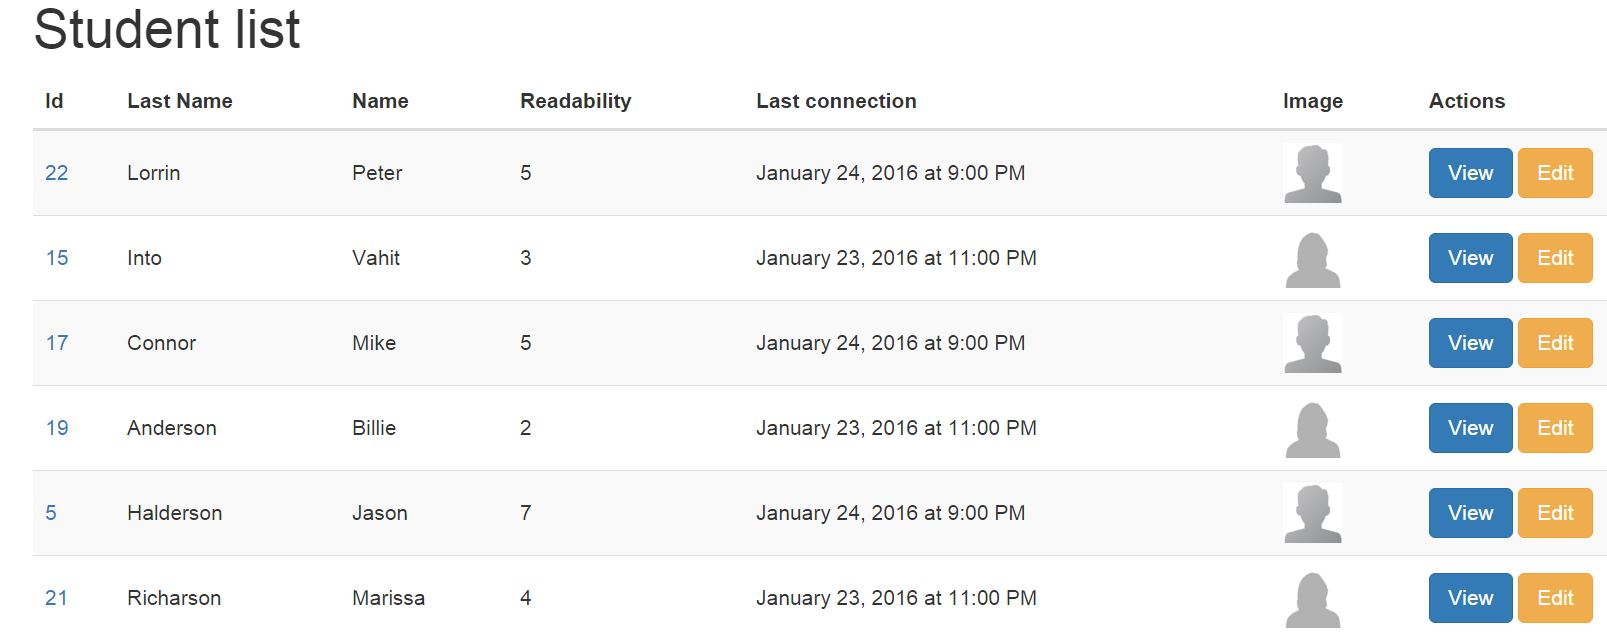
\includegraphics[width=1\textwidth]{StudentList}
 \caption{Screenshot of student list for educator}
  \label{fig:studentList}
 \end{figure*}
\section{Introduction}


K-12 students make use of the internet in a daily basis seeking materials that can help them with their academic tasks, such as finding information for a class presentation or discovering the meaning of a new word. For this purpose, they often turn to search engines and online available catalogs for retrieving reading materials that can satisfy their information needs, including news articles, books or term definitions. However, they can often get discouraged because the contents they retrieve are outside their comprehension level, whether being too easy or too difficult  for them to read, thus, helping them to seek for adequate materials they can actually comprehend is imperative.\\

%Reading is an important skill in the academic environment, a skill that can have a high impact for a student's educational opportunities and their career \cite{robinson2000issues}. However, students can get discouraged to read, when the texts provided are outside of their comprehension level, whether being too easy to read  or too difficult for them.


In the academic environment students are not the only ones facing the problem of locating adequate reading materials that simultaneously match the information needs and reading abilities of an individual. Educators also face several challenges when looking for materials for their classes, making them spend a significant amount of their time doing so. For example, even in a same grade class, students' reading skills can differ significantly, so not all students in the same class can be provided with same texts. This supposes a personalization need that the instructor has to handle on a daily basis. However with the high number of students in class this task can become impossible to tackle. \\



%Due to the mentioned fact, instructors spend a significant amount of their time seeking adequate materials for their students, a time that could be reduced with the help of an specialized application.\\


\textit{YouUnderstood.me} is a web application oriented to both instructors and students that aims at helping them in the process of finding reading materials. The system is centered on the use of readability formulas that together with a search engine makes looking for levelled reading material fast and efficient. \textit{YouUnderstood.me} lets students log in in the application, which keeps track of  feed-back they have given for each of the read materials (too easy/OK/too complex). This enables the application to make predictions about the readability score for each student, and give both the student and his educator, the possibility to see an updated readability score that can be helpful for speeding-up the process of searching adequate materials. Furthermore, the application contains a search engine that allows both students and educators to seek materials filtered by readability score from: (i) commercial search engines, such as google, (ii) public data sources, such as Wikipedia and (iii) local resources, such as the catalogues of a school library.\\

%, AR\footnote{http://www.acceleratelearning.com} or Lexile\footnote{http://lexile.com} 

Finally, the instructors also have access to an analysis page, where they can submit texts they found outside the application for determining their readability score, being able to choose from a wide range of readability formulas provided within the application. This tool, together with the track of readability scores of each students, helps teachers make sure the reading materials they found are adequate or not for the class.\\

The novelty of \textit{YouUnderstood.me} lays in how the different modules are combined in order to create an application that becomes helpful in an academic environment. To the best of our knowledge, \textit{YouUnderstood.me} is the first application that tackles the issue of reading material retrieval as a whole. Starting from the assessment of an individual student's readability, and ending with the retrieval of adequate materials, all modules of \textit{YouUnderstood.me} work in cooperation in order to speed-up the process of reading material selection.

 

\section{YouUnderstood.me}
Whether when a student is searching information for completing an assignment or when an educator uses the application for finding material for his course, a text's complexity needs to be determined in order to evaluate if the material fits the needs of readability level.\\




Different approaches have been followed in the literature for determining a text's complexity or readability. Most approaches, focus their work in determining the readability of a general text. Those systems vary, from the very simple ones \cite{flesch1948new}, which make use of shallow features, such as, the average number of words per sentence or the average length of terms, to more complex ones \cite{gonzalez2014simple}\cite{dell2011read} \cite{franccois2012ai}, which are mostly based, on supervised learning techniques and features extracted using Natural language processing. However, those tools have shown to be of small use in contexts where the text of the reading material has reduced accessibility, both because the texts is not publicly accessible or because it shows a structure that is not as simple to tackle . Therefore, different works have been done in more specialized contexts such as book \cite{denning2015readability}\cite{pera2014automating} or web page retrieval [Ref], where the systems presented made use other features apart from the ones in the text.\\


\textit{YouUnderstood.me} can make use of different readability assessment metrics and resources at the same time, aiming to be able to handle a more diverse amount of reading materials. The methods with which  \textit{YouUnderstood.me} can assess a reading material readability are the following:

\begin{itemize}
\item \textbf{External metrics.} \textit{YouUnderstood.me} is compatible with the most popular readability metrics among the American education centers and libraries, such as the ones that are used in material catalogs like AR or Lexile. The compatibility with those types of metrics allows the application to be able to retrieve books, which have been historically an issue for readability formulas, because of the inability to get access to the contents of copyrighted material \cite{denning2015readability}.
\item \textbf{Traditional formulas.} Historically used by teachers for manually determining the readability level of a reading material, traditional formulas such as Flesh \cite{flesch1948new}, Fog\cite{gunning1952technique} and Flesh-Kincaid \cite{flesch1948new}, are supported by \textit{YouUnderstood.me}. These formulas enable educators compare new materials with the old, hand-way measured materials they may have stored during their teaching career.
\item \textbf{MRAS.} MRAS \cite{imadrazo2016readability} (Multilingual Readability assessment system) is a state of the art readability assessment system, that is capable of detecting the input language of a text on the fly and providing a readability score for it. MRAS is based on a supervised learning paradigm, at the moment, makes use of more than a hundred features for learning and prediction. The features are extracted using Natural Language Processing tools, such as a tokenizer, a part of speech tagger and different semantic analyzers. Those features, are used to train a model that will later be used for predicting the readability score for new materials.


\end{itemize}

The stakeholders of \textit{YouUnderstood.me} can benefit of the aforementioned readability scores in different ways. On the one side, \textbf{students} can make use of a \textbf{search engine} (fig. \ref{fig:studentSearch}) which provides several features that are aimed at helping the student in the process of seeking an adequate reading material. In order to use it, the student needs to be logged in (a), which permits the application personalize the experience the student is having by different means.\\

Each query a student inserts is first treated with {\color{red} OSIM (Our search intent module)[Ref]}, an ad-hoc developed search intent module for children. OSIM is capable of treating issues that usually arise while processing children queries, such as misspelling, children popular culture terms or too long queries [Ref]. Issues that usually lead children to get poor results while using a common search engine.\\

Once the query is treated and converted into a new query, it is submitted to the corresponding search tool. Currently two methods of search are implemented: a method that makes use of the Google Search API and a method based the lucene framework.
\\

Once results are retrieved by the corresponding search engine, they are analyzed for their readability and filtered by the readability requirements of each individual student. The documents can be both dynamically or statically analyzed, depending on their source and the search tool used. For example, the documents need to be analyzed on the fly when using Google, since the documents are not in possession of the application. This supposes that the readability prediction needs to be fast, forcing the application to use a lightweight readability formula such as Flesch or FOG. However, when using Lucene, the documents can be previously analyzed, enabling the use of more complex readability prediction tools, such as MRAS.\\


Once the student has read the chosen material, he can give feed-back on it (c), helping the system improve the recommendations for future searches. This feed-back is given by means of a three option question which permits the student state whether the reading material was too easy, OK, or too complicated. This information is provided to the tracking system in order to create predictions about individual users' readability skills.\\ 

The \textbf{tracking system} is currently based on a trivial method of approximation which simply increases the student's readability score every time he finds a recommended reading material too easy, and decreases it, every time he finds it too complicated. However, we are conscious that more precise methods exist and plan to implement them in the near future. An updated prediction of the system regarding each student can be seen on the profile menu (d), permitting each student keep track of the progress he is making.\\



\textbf{Educators} can also make use of the \textbf{search engine} interface, which is adapted to their use (fig. \ref{fig:educatorSearch}). The educator view of the search engine does not require the educator to be logged in, giving the user himself the possibility of personalizing the searches. The search engine no longer makes use of the search intend module, given that the educators are supposed to find the correct words for what they are seeking, and adding this extra layer of filtering would only hinder their work. Furthermore, the readability level for filtering the reading materials is no longer decided by the system, giving the educator the option for choosing the level of challenge he want for his students. The feed-back options are no longer available either, since there is no point in evaluating the educator's readability.\\


\textbf{Educators} can also make use of the material analysis page (fig. \ref{fig:analysispage}). This page, permits educators analyze reading materials they cannot find using the provided search engine, i.e. when materials are self created. This tool allow to choose the readability formula used for the analysis, among all the formulas that have already been mentioned.

%TODO change image, add posibility to choose formula
\begin{figure}[h!]
 \centering
  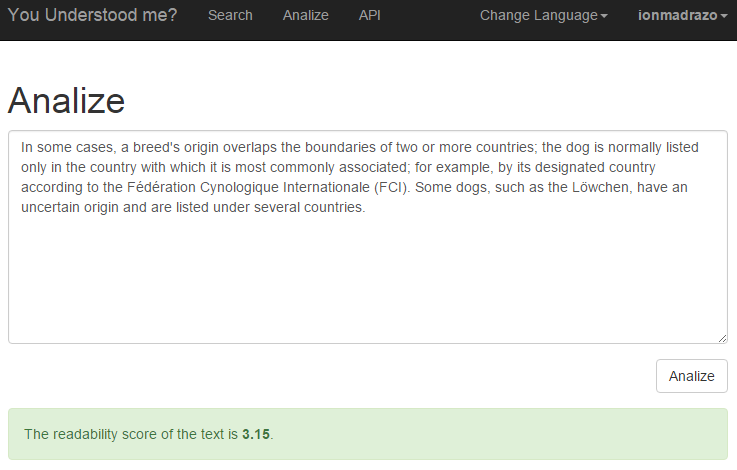
\includegraphics[width=0.5\textwidth]{AnaliseScreenShot2}
 \caption{Screen shot of analysis page}
 \label{fig:analysispage}
 \end{figure}
 
 
 
Finally, a student tracking tool is provided for educators (fig. \ref{fig:studentList}). This tool provides a fast way to know the individual and overall reading skills of the students in the  class. The educator can view a prediction for individual student's reading skills or go deeper and view the feed-back that the student gave for each of the read materials.




%The document analyzer is the center of the the application
%It is used for both analysis tool and material searcher
%





%Where does it work, catalogs, internet, enciclopedias
%How does it work, search filtering?



\begin{comment}
\section{User Experience}

\begin{itemize}
\item \textbf{Analyzing materials.} An analysis page is provided to instructors, so that they can make use of the readability assessment algorithm \cite{imadrazo2016readability} with materials from outside the application. This page provides an input form where the instructor can submit the material, and receive a readability level prediction for the it.


\item \textbf{Looking for new materials.} A material search page is provided so that the user can insert text queries for looking for materials. The user can select a certain readability level he wants to look for, of leave it blank letting the application choose the best level for the logger user. Furthermore, the material source can be selected, depending on the user needs. In case of students, they can select a material for reading and provide feed-back on it. This feed-back will be used for tracking purposes.


\item \textbf{Tracking students.} The educator can see a table with data about all his students, where the number of materials read and the readability score for each student are provided. The instructor can go deeper if needed, and see each of the materials each students has read and the individual readability scores for each material, as well as, the feed-back given by the student. The data is also presented in a summarized way, so that the educator can see the average, maximum and minimum reading skills of the students in class.

\end{itemize}

\end{comment}

\section{Conclusion and Future work}



\bibliography{bibliography}{}
\bibliographystyle{apalike}
\nocite{*}
\end{document}
